\chapter{Validation, Traction, and the Scalable Startup}

This lecture is conversational rather than blackboard-based, yet it has a definite mathematical spine. We are led from entrepreneurial folklore to a founder's sequence of operating tests: validate the market before we build, distinguish a real problem from a scalable business, accept feedback before perfection, raise capital only after traction begins to repeat, and scale by spending founder time where it has the highest leverage. The formalism in this chapter is therefore organizational rather than physical. We write down a few inequalities and logical chains not as theorems of finance, but as compact versions of the decision rules that the interview keeps returning to. The governing idea is simple: market first, product second, capital later, scale after proof.

\section{Opening Montage and Entrepreneurial Stakes}

\paragraph{Anecdote.} The lecture begins in motion. We are on the way to meet John Abraham, and before the main conversation settles, the video runs through a teaser montage of questions about capital, past exits, rejection, networking, and wealth.

\paragraph{Claim.} Even in this opening prelude, the lecture announces two large themes. First, outsized wealth is tied to ownership rather than wages alone. Second, business progress is not merely transactional; it depends on durable relationships and repeated contact with reality.

We can compress the opening wealth claim into a heuristic relation:
\begin{equation}
\text{path from seven to eight figures}
\;\approx\;
\text{equity in somebody else's company}
\;\;\text{or}\;\;
\text{equity in one's own company}.
\end{equation}

\paragraph{Mechanism.} The montage does not yet tell us how to build such ownership. It merely marks the questions that the rest of the lecture will answer more carefully: how to start, how to validate, how to fund, how to scale, and how to make a company worth buying.

\section{From Public Advice to the Founder Case}

\paragraph{Anecdote.} Before the main founder interview, the lecture passes through street-level business talk: a retired tech salesman describes eight-figure wealth from stock options, a government consultant emphasizes relationships over networking, and another business owner praises niche selection and fast exits from bad bets. The hosts also recount rejection on the street and the rule that every no moves us closer to a yes.

\paragraph{Claim.} These public fragments matter because they create the background noise of entrepreneurship: ownership, rejection, niche positioning, and the social character of business. But the lecture does not leave us there. It pivots back to a more stable case.

The hosts explain that they first overheard Abraham discussing business in an Austin restaurant, then returned later to record a fuller conversation. That transition matters. We move from general entrepreneurial atmosphere to a witness who has actually launched, exited, and started again.

\paragraph{Anecdote.} Abraham's own chronology is concise:
\begin{equation}
t_{\text{launch}} = 2014,
\qquad
t_{\text{exit}} = 2018.
\end{equation}
He began in tech sales, launched an application, exited four years later, and is now building Haymaker, a marketplace for temporary office and meeting space.

\paragraph{Mechanism.} This timeline is not decoration. It supplies the authority for the lecture's main methodological claim: entrepreneurial judgment is not a single act of inspiration, but a repeatable sequence of tests.

\section{Validate Before We Build}

\begin{definition}
We use \(\mathrm{TAM}\) for the total addressable market. In this lecture it is not computed numerically; it serves as a discipline. Before we build, we ask whether the problem we see belongs to a market large and concrete enough to sustain a company.
\end{definition}

\begin{definition}
We use \(\mathrm{MVP}\) for the early product built after some market evidence appears. Abraham says ``minimally viable product.'' The abbreviation is standard; the important point is sequence rather than vocabulary.
\end{definition}

\paragraph{Anecdote.} The host asks the first serious operating question: how do we turn a good idea into action?

\subsection{Question \& Answer}

\paragraph{Question.} What is the first step from idea to execution?

\paragraph{Answer.} The lecture's answer is deliberately anti-romantic. Before creating anything, we should understand the viability of the product and the \(\mathrm{TAM}\). Then we should interview as many potential clients as possible, especially decision-makers in the relevant space.

\paragraph{Mechanism.} The operating chain can be written compactly as
\begin{align}
\text{Need observed}
&\Rightarrow \text{interview decision-makers},\\
\text{Interview evidence}
&\Rightarrow \text{clearer statement of pain},\\
\text{Pain with business value}
&\Rightarrow \text{pilot commitment},\\
\text{Pilot commitment}
&\Rightarrow \text{build the }\mathrm{MVP}.
\end{align}

The lecture is especially careful at one point: we do not begin by forcing a sale. We begin by asking what the client's current challenges are and what solving them would mean for the business. Only after that conversation matures do we ask for something stronger, namely a willingness to pilot the solution.

\begin{figure}
\centering
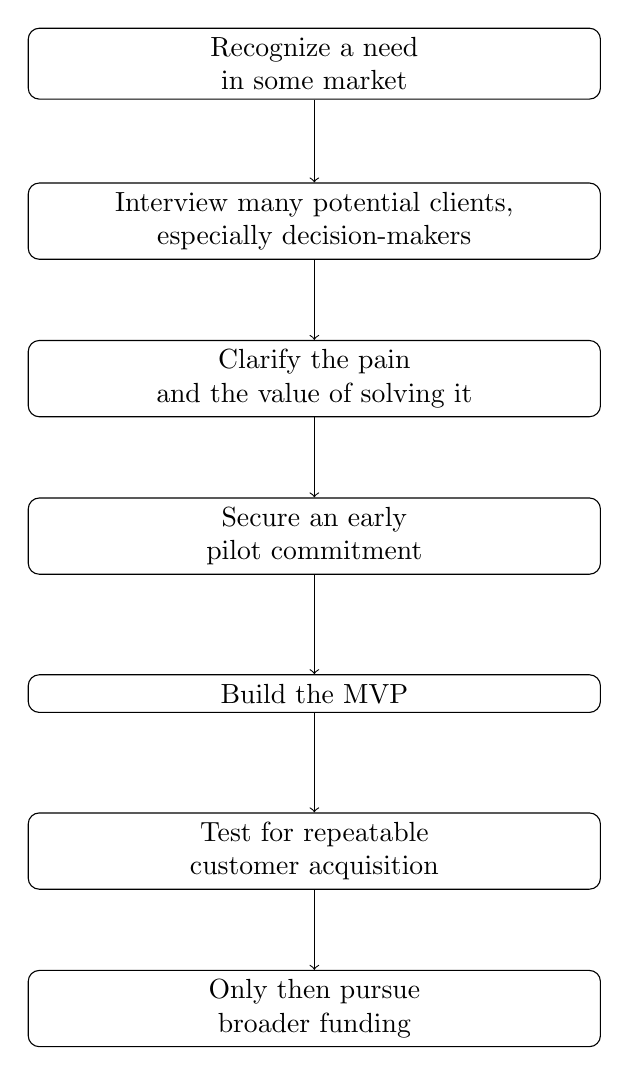
\begin{tikzpicture}
\node[draw, rounded corners, align=center, text width=0.58\linewidth] (n1) at (0,0) {Recognize a need\\in some market};
\node[draw, rounded corners, align=center, text width=0.58\linewidth] (n2) at (0,-2.0) {Interview many potential clients,\\especially decision-makers};
\node[draw, rounded corners, align=center, text width=0.58\linewidth] (n3) at (0,-4.0) {Clarify the pain\\and the value of solving it};
\node[draw, rounded corners, align=center, text width=0.58\linewidth] (n4) at (0,-6.0) {Secure an early\\pilot commitment};
\node[draw, rounded corners, align=center, text width=0.58\linewidth] (n5) at (0,-8.0) {Build the \(\mathrm{MVP}\)};
\node[draw, rounded corners, align=center, text width=0.58\linewidth] (n6) at (0,-10.0) {Test for repeatable\\customer acquisition};
\node[draw, rounded corners, align=center, text width=0.58\linewidth] (n7) at (0,-12.0) {Only then pursue\\broader funding};

\draw[->] (n1) -- (n2);
\draw[->] (n2) -- (n3);
\draw[->] (n3) -- (n4);
\draw[->] (n4) -- (n5);
\draw[->] (n5) -- (n6);
\draw[->] (n6) -- (n7);
\end{tikzpicture}
\end{figure}

\begin{remark}
There is no claim here that the lecture produced a literal board derivation. The chain above is a faithful condensation of the spoken sequence.
\end{remark}

\section{When Does an Idea Become Good Enough?}

\paragraph{Anecdote.} The next question is exactly the right one. Suppose we have an idea, a team, and some money going out the door. At what point do we know we should keep investing?

\subsection{Question \& Answer}

\paragraph{Question.} When is an idea good enough to deserve more time and more capital?

\paragraph{Answer.} Abraham's answer is sharp: not when the problem merely sounds substantial. The idea is not yet good in the entrepreneurial sense until we know how to get customers at scale.

That distinction can be written as
\begin{equation}
\text{Substantial problem alone}
\;\not\Rightarrow\;
\text{great business}.
\end{equation}
More positively,
\begin{equation}
\text{Great business idea}
\;\Rightarrow\;
\bigl(\text{substantial problem}\bigr)
\land
\bigl(\text{customer acquisition can scale}\bigr).
\end{equation}

\paragraph{Mechanism.} This is the lecture's first genuinely strict gate. We are not allowed to confuse importance with distribution. A painful problem may exist, and yet the business may still fail if there is no repeatable path from product to paying customer. In that sense the question ``Is this a good idea?'' is really shorthand for the harder question ``Can this problem be turned into a repeatable customer-acquisition machine?''

\section{Perfectionism, Failure, and the Feedback Loop}

\paragraph{Anecdote.} Once the lecture has tied judgment to the market, it immediately turns to the founder pathologies that resist market contact. The host asks about perfectionism, analysis paralysis, and the fear of sending a product out before it is finished. A little later he asks about repeated failure and setbacks.

\paragraph{Claim.} Abraham's diagnosis is severe and useful. Perfectionism is treated not as craftsmanship but as insecurity: we do not want anyone calling the baby ugly, so we never show them the baby. The lecture is warning us that excessive inward refinement can be the enemy of external learning.

We can express the contrast schematically:
\begin{align}
\text{imperfect release}
&\Rightarrow \text{feedback}
\Rightarrow \text{course correction},\\
\text{hidden product}
&\Rightarrow \text{no feedback}
\Rightarrow \text{no correction}.
\end{align}

\paragraph{Mechanism.} The same structure explains the later discussion of adversity. Rejection is not noise outside the process; it is part of the process. The early street-interview segment prepares us for this point. The founder who can survive criticism, rejection, and partial failure is not merely enduring pain. He is collecting the information required for the next correction.

\paragraph{Claim.} The lecture then widens the frame. Entrepreneurship is not the destination; it is the journey that shapes the operator. Money from an exit or an IPO may be the public sign, but the deeper transformation comes from learning to meet obstacles head-on and continuing anyway.

\section{Capital, Traction, and Scaling Rules}

\paragraph{Anecdote.} The lecture now returns to one of the teaser questions from the opening montage: how do we raise capital efficiently?

\subsection{Question \& Answer}

\paragraph{Question.} What do investors really need to see before funding a young business?

\paragraph{Answer.} The lecture refuses a magic threshold. There is no sacred number at which a company becomes fundable. Instead, the founder must show a cluster of signals: potential, repeatable customer acquisition, and a plan.

We can write the rule as
\begin{equation}
\text{Ready for investment}
\;\Rightarrow\;
\bigl(\text{potential}\bigr)
\land
\bigl(\text{repeatable acquisition}\bigr)
\land
\bigl(\text{plan}\bigr).
\end{equation}

\paragraph{Mechanism.} The order is crucial. First we build and test as cheaply as we can. Then, if possible, we generate revenue. Then we reinvest into broader traction. Only after that do we take the company out for outside investment.

The lecture adds one lightly quantitative refinement. Ideally the operating data should be moving upward month by month:
\begin{align}
R_{t+1} &> R_t,\\
\mathrm{MRR}_{t+1} &> \mathrm{MRR}_t.
\end{align}
Here \(R_t\) denotes period revenue and \(\mathrm{MRR}_t\) monthly recurring revenue at period \(t\).

\begin{remark}
These inequalities are not quoted board formulas from the lecture. They are cautious symbolic versions of Abraham's verbal criterion that revenue and recurring revenue should be moving upward.
\end{remark}

\paragraph{Anecdote.} The host then asks how we scale from one revenue band to the next. Abraham answers with an operational rule, not a grand theory.

Let \(r_F\) denote the founder's effective hourly rate and \(c_{\text{task}}\) the outside cost of a task. Then the lecture's scaling rule can be written as
\begin{equation}
c_{\text{task}} < r_F
\;\Rightarrow\;
\text{outsource the task}.
\end{equation}

\paragraph{Mechanism.} This rule does two things at once. It protects founder time for higher-leverage work, and it forces the company to estimate what founder time is actually worth. If the task cannot be outsourced cleanly and instead requires a permanent hire, the lecture insists on forecast discipline: put the role in the budget, build it into the plan, and expand deliberately rather than by improvisation.

\section{Go-to-Market, Saleability, Advisors, and Haymaker}

\paragraph{Anecdote.} After capital and scaling, the lecture shifts into business architecture: go-to-market strategy, exit preparation, mentor structure, and finally the specifics of Haymaker itself.

\paragraph{Claim.} Marketing is not monolithic. The channel mix depends on what kind of business we are running. In the lecture the split is simple and practical:
\begin{align}
\text{Enterprise play}
&\Rightarrow \text{email + direct outreach + possibly cold calling},\\
\text{Consumer play}
&\Rightarrow \text{social media plays a critical role}.
\end{align}

\paragraph{Mechanism.} This is consistent with the earlier validation logic. The lecture never treats marketing as decoration. Channels are chosen by buyer type, and buyer type was already implicit in the earlier insistence that we talk to decision-makers.

\paragraph{Claim.} The same disciplined thinking governs exits. The best way to make a company saleable is not to perform for acquirers. It is to keep building revenue and moving the bottom line efficiently, so that investors or acquirers notice a machine worth joining or buying.

We can write the operating claim schematically as
\begin{equation}
\text{efficient revenue growth}
\;\Rightarrow\;
\text{investment or acquisition attention}.
\end{equation}

\paragraph{Mechanism.} The lecture is equally careful about advisors. There is usually not one mentor for everything. Motivation may come from one person, but domain guidance must come from domain experts. In other words, advisory structure should mirror the differentiated structure of the business itself.

\paragraph{Anecdote.} The chapter then closes by returning to a concrete venture. Haymaker is described as a marketplace, comparable in form to Airbnb, but aimed at temporary office and meeting spaces. The company pivoted from a coworking emphasis toward meeting spaces as the pandemic and distributed work reduced the appetite for large permanent footprints. This is an important ending. We return from abstract rule to a live example of market observation, repositioning, and fit.

\section{Summary}

The lecture's logic is sequential and disciplined. We begin with a market need, not a private attachment to an idea. We test that need through interviews with decision-makers, clarify what solving the problem would mean, seek a pilot, and only then build the \(\mathrm{MVP}\). We do not call an idea good simply because the problem is real; we call it promising only when customer acquisition begins to look scalable. We do not wait for perfection, because hidden products cannot teach us anything. We do not raise capital from mythology or from a magic number, but from evidence of potential, repeatable acquisition, a plan, and ideally rising revenue and \(\mathrm{MRR}\). And when the business begins to scale, we protect founder time, choose channels by buyer type, and make the company saleable by running it efficiently.

This is the chapter's durable contribution to the book. The lecture is not a collection of startup slogans. It is a compact operating philosophy: validate first, prove traction next, fund after evidence, and scale through leverage, specialization, and clear contact with the market.